\documentclass[12pt]{ociamthesis}  % default square logo 
%\documentclass[12pt,beltcrest]{ociamthesis} % use old belt crest logo
%\documentclass[12pt,shieldcrest]{ociamthesis} % use older shield crest logo

%load any additional packages
\usepackage{amssymb}
\usepackage{amsmath}
\usepackage{longtable}
\usepackage{float}
\usepackage{listings}


%input macros (i.e. write your own macros file called mymacros.tex 
%and uncomment the next line)
%\include{mymacros}

\title{Laporan Tugas\\[1ex]     %your thesis title,
        Chapter III}   %note \\[1ex] is a line break in the title

\author{Muhammad Wahyu Ardi Ismail}             %your name
\college{NPM : 1.18.4.059 }  %your college

%\renewcommand{\submittedtext}{change the default text here if needed}
\degree{Applied Bachelor Program of Informatics Engineering}     %the degree
\degreedate{Bandung 2019}         %the degree date

%end the preamble and start the document
\begin{document}

%this baselineskip gives sufficient line spacing for an examiner to easily
%markup the thesis with comments
\baselineskip=18pt plus1pt

%set the number of sectioning levels that get number and appear in the contents
\setcounter{secnumdepth}{3}
\setcounter{tocdepth}{3}


\maketitle                  % create a title page from the preamble info
%\begin{dedication}
`Jika Kamu tidak dapat menahan lelahnya belajar, \\
Maka kamu harus sanggup menahan perihnya Kebodohan.'\\ 
~Imam Syafi'i~\\
\end{dedication}        % include a dedication.tex file
%\begin{acknowlegements}
Pertama-tama kami panjatkan puji dan syukur kepada Allah SWT yang telah memberikan rahmat dan hidayah-Nya sehingga Laporan Tugas Chapter I Pemrogaman II dapat terselesaikan dengan tepat waktu. Tidak lupa penulis mengucapkan shalawat serta salam kepada nabi junjungan kita Nabi Muhammad SAW.

Laporan ini disusun untuk memenuhi kelulusan matakuliah Pemrogaman II pada Program Studi DIV Teknik Informatika. Proses Laporan Tugas Pemrogaman II ini juga tidak terlepas dari bantuan berbagai pihak. Oleh karena itu, pada kata pengantar ini penulis menyampaikan teriamakasih kepada :
\begin{enumerate}

\item kepada Allah SWT yang telah memberikan rahmat serta bantuanya sehingga laporan tugas chapter 1 pemrogaman II ini dapat selesai tepat waktu;
\item  kepada Bapak/Ibu yang selalu memberikan dukungan baik moral ataupun spiritual;
\item	Kepada Rolly Maulana Awangga, S.T., M.T.I. selaku Dosen Pembimbing Pemrogman II Tahun Akademik 2019/2020;
\item	M. Yusril Helmi Setyawan, S.Kom., M.Kom. selaku Ketua Program Studi DIV Teknik Informatika Tahun Akademik 2018/2019;
\item	Dr. Ir. Agus Purnomo, M.T. selaku Direktur Politeknik Pos Indonesia Tahun Akademik 2018/2019.

\end{enumerate}

Penulis telah membuat laporan ini dengan sebaik-baiknya, diharapkan memberikan kritik dan saran dari semua pihak yang bersifat membangun, terimakasih.
\end{acknowlegements}   % include an acknowledgements.tex file
%\begin{abstract}
	Panduan Penulisan Jurnal Ilmiah (PPJI) ini dibuat dengan tujuan memberikan acuan bagi para sivitas akademika
	yang memulai menulis jurnal ilmiah. Pada intinya PPJI menjelaskan secara lengkap tentang standar pengerjaan jurnal internasional dari pengalaman penulisan dari tahun 2017. Di dalamnya memuat aturan standar penulisan dan penggunaan Latex sebagai editor. Dengan demikian diharapkan semua sivitas akademika dapat membuat jurnal ilmiah dengan
	 lancar dan sesuai dengan standar.
\end{abstract}          % include the abstract

\begin{romanpages}          % start roman page numbering
%\tableofcontents            % generate and include a table of contents
%\listoffigures              % generate and include a list of figures
\end{romanpages}            % end roman page numbering

%now include the files of latex for each of the chapters etc
\chapter*{Teori}

\begin{enumerate}
	\item CSV(Comma Separated Value) adalah format data yang digunakan para pengguna untuk menginputkan data kedalam database secara sederhana.

	\begin{itemize}
	\item Fungsi file CSV adalah format basis data sederhana yang di setiap record dipisahkan dengan tanda koma dan titik koma.
	\end{itemize}
	
	\begin{figure} [h]
	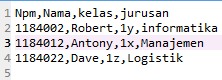
\includegraphics[width=5cm]{poto/1.png}
	\centering
	\end{figure}		
	
	
	
	
	\item Aplikasi yang dapat membuat file CSV adalah Notepad,Worpad,Microsoft Excel,dll
	
	\item Cara membuat file CSV:
	\begin{itemize}
	\item Buka Ms.Excell
	\end{itemize}
	\begin{itemize}
	\item Membuat data di Ms.Excel
	\end{itemize}
	\begin{itemize}
	\item Lalu pada saat menyimpan pilih "save as" dan jenis file nya diganti csv
	\end{itemize}
	\begin{itemize}
	\item Dan file CSV telah dibuat
	\end{itemize}

	\item library csv adalah format yang sudah digunakan selama bertahun-tahun dengan cara standar di RFC 4180. Perbedaan halus terdapat di beberapa aplikasi.
	
	
	\item library Pandas adalah alat analisis data dan struktur unruk bahasa pemrograman Python.  Panda digunakan dengan mudah untuk mengelola data salah satu fiturnya adalah Dataframe. Dataframe dapat digunakan untuk membaca sebuah file dan menjadikannya table.


	\item Fungsi yang terdapat pada library CSV:\\
	\begin{itemize}
	\item Reade, Fungsi Reader diguunakan untuk membaca  isi file
	\end{itemize}
	\begin{itemize}
	\item Dict Reader, Fungsi Dict Reader digunakan untuk membaca isi file yang terdapat di dictionary
	\end{itemize}
	\begin{itemize}
	\item Write, Fungsi Write ini digunakan untuk menulis file
	\end{itemize}
	\begin{itemize}
	\item Dict Write, Fungsi Dict Write digunakan untuk menulis file yang ada di dictionary
	\end{itemize}
	
	\item Fungsi yang terdapat di libarary pandas
	\begin{itemize}
	\item to\_csv, untuk menulis file yang type nya CSV
	\end{itemize}
	\begin{itemize}
	\item read\_csv, untuk membaca file type CSV
	\end{itemize}
	
	
\end{enumerate}




%next line adds the Bibliography to the contents page
\addcontentsline{toc}{chapter}{Bibliography}
%uncomment next line to change bibliography name to references
%\renewcommand{\bibname}{References}
\bibliography{references}        %use a bibtex bibliography file refs.bib
\bibliographystyle{plain}  %use the plain bibliography style

\end{document}

